 \chapter{偶极辐射与散射}\label{ch:b2:dipole-radiation}

天空为什么是蓝色的，为什么它在与太阳成直角的方向上最蓝
——并且在那里是偏振的，蜜蜂和摄影师对此心知肚明？为什么一座
无线电发射塔必须高数十米，它为何
正上方什么也不辐射？两个问题的答案相同：一个
振荡电荷辐射\omterm{thm:b2:plane-waves-polarization:wave}{电磁波}，其
功率随频率的四次方增长，\omterm{prop:b2:dipole-radiation:power}{辐射方向图}
沿振荡轴消失。
本章给出\emph{\omterm{thm:b2:dipole-radiation:field}{振荡偶极子}}的场，它是最简单的辐射系统，
由此导出天线及加速电荷的辐射，
并将其应用于空气分子，每个分子都是一根微小天线，
重新发射太阳光：\omterm{prop:b2:dipole-radiation:rayleigh}{瑞利散射}。

\begin{omfigure}
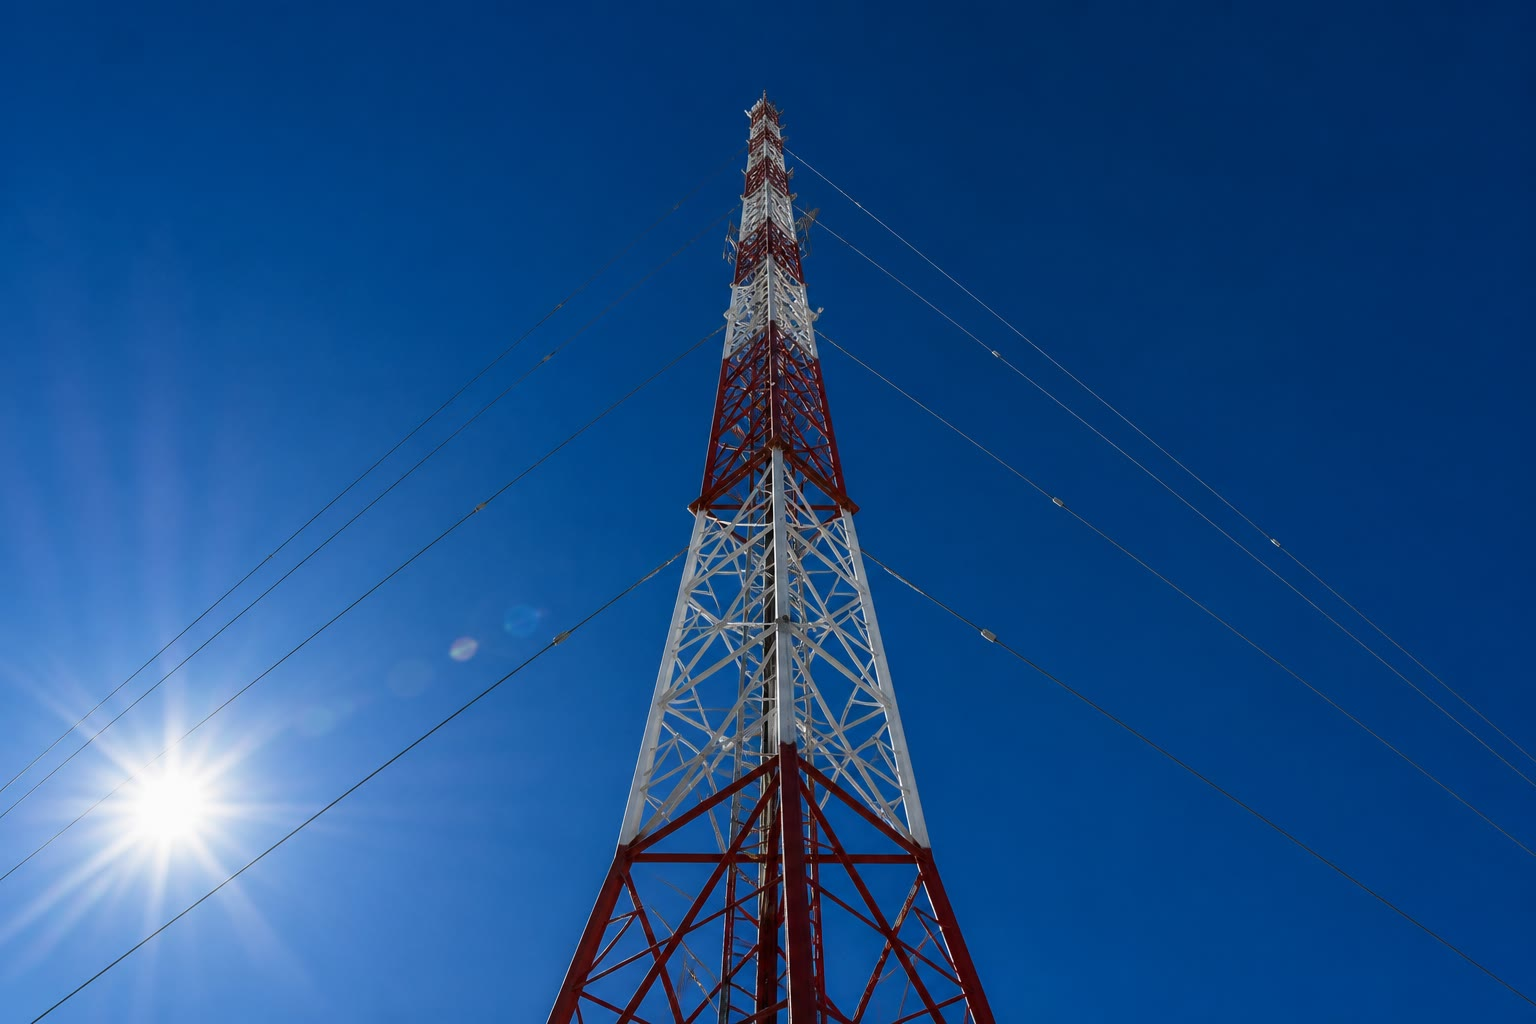
\includegraphics[width=0.54\linewidth]{images/book4/ai/b4-17-radio-mast-blue-sky.jpg}

{\small 蓝天下的广播发射塔：一根高数十米的竖直偶极子向地平线辐射，其上方的天空被数十亿个分子偶极子照亮，它们再辐射太阳光。}
\end{omfigure}


\section{振荡偶极子的场}

\begin{theorem}[电偶极子的辐射场]\label{thm:b2:dipole-radiation:field}
\index{振荡偶极子}\index{辐射区}\index{推迟}
偶极矩为 $\vect p(t) = p_0\cos\omega t\,\vect e_z$、尺度为 $a$ 的偶极子，位于
原点并辐射。在\emph{\omterm{thm:b2:dipole-radiation:field}{辐射区}}——即距离 $r \gg
\lambda = 2\pi c/\omega \gg a$ 处——其场在球坐标 $(r,
\theta, \varphi)$（以偶极子的轴为极轴）为
\[
\vect E(M, t) = -\frac{\mu_0\,\omega^2p_0}{4\pi}\,\frac{\sin\theta}r\,\cos\bigl(\omega(t - r/c)\bigr)\,\vect e_\theta ,
\qquad
\vect B = \frac{\vect e_r\wedge\vect E}c :
\]
一个\omterm{prop:b2:sound-waves:spherical}{球面波}，局部为平面波——$(\vect E, \vect B, \vect e_r)$ 是一个
右手标架，且 $B = E/c$——其场被传播时间
$r/c$ 所\emph{\omterm{thm:b2:dipole-radiation:field}{推迟}}，振幅随 $1/r$ 衰减，与偶极子的加速度
$\ddot p = -\omega^2p$ 成正比，并与 $\sin\theta$ 成正比：在
赤道面内最大，沿轴线为零；偏振面位于
包含轴线的平面内。
\end{theorem}
\admitted

\begin{remark}[读懂公式]\label{rem:b2:dipole-radiation:reading}
\omterm{thm:b2:maxwell-equations:maxwell}{麦克斯韦方程组}的精确解（由\omterm{thm:b2:dipole-radiation:field}{推迟}势得出，
超出本卷范围）还含有 $1/r^2$ 与
$1/r^3$ 项；后者即本科一年级分册中的准静态偶极子场，
$\vect E \propto p/4\pi\varepsilon_0r^3$，它在\emph{近
区} $r \ll \lambda$ 中占主导；在 $r \sim \lambda/2\pi$ 处两项相当，超过此距离后
只有 $1/r$ 项保留。各因子都有其理由。$1/r$：
通过球面的功率 $\propto E^2r^2$ 不能依赖于 $r$。$\omega^2p_0$：
静止或匀速运动电荷的场不具辐射性；它
辐射的是\emph{加速度}。$\sin\theta$：位于轴线上的观察者
看到沿视线来回运动的电荷，没有横向加速度；
而在赤道面内，整个加速度都是横向的。
\omterm{thm:b2:dipole-radiation:field}{推迟}：$M$ 点在时刻 $t$ 的场
反映的是偶极子在 $t - r/c$ 时刻的状态。
\end{remark}

\begin{omfigure}
\begin{tikzpicture}[font=\small, x=1cm, y=1cm, >=Stealth]
  \begin{scope}
    \draw[->, thick] (0,-2.2) -- (0,2.4) node[right, font=\footnotesize] {$z$};
    \draw[omThm, very thick, <->] (0,-0.5) -- (0,0.5); \node[omThm, font=\footnotesize] at (0.35,0.0) {$\vect p$};
    \coordinate (M) at (2.6,1.6);
    \draw[dashed] (0,0) -- (M); \fill (M) circle (1.5pt); \node[font=\footnotesize] at (2.45,1.25) {$M$};
    \draw (0,0.7) arc[start angle=90, end angle=31.6, radius=0.7]; \node[font=\footnotesize] at (0.35,0.9) {$\theta$};
    \draw[omDef, very thick, ->] (M) -- ($(M)+(0.55,-0.9)$) node[right, font=\footnotesize] {$\vect E$ ($\vect e_\theta$)};
    \node[omProp, font=\footnotesize] at ($(M)+(-0.65,0.25)$) {$\vect B$ $\otimes$};
    \draw[omExo, thick, ->] (M) -- ($(M)+(0.7,0.43)$) node[right, font=\footnotesize] {$\vect e_r$};
    \node[font=\footnotesize] at (0,-2.7) {$E \propto \dfrac{\omega^2p_0\sin\theta}{r}\cos\omega(t - r/c)$};
  \end{scope}
  \begin{scope}[xshift=8.6cm]
    \draw[->, thick] (0,-2.2) -- (0,2.4) node[right, font=\footnotesize] {$z$};
    \draw[omThm, thick, domain=0:360, samples=120, smooth] plot ({2.0*sin(\x)*sin(\x)*sin(\x)},{2.0*sin(\x)*sin(\x)*cos(\x)});
    \draw[omThm, very thick, <->] (0,-0.35) -- (0,0.35);
    \node[omThm, font=\footnotesize] at (2.3,0.35) {$\sin^2\theta$};
    \node[font=\footnotesize] at (0,-2.7) {单位立体角内的辐射功率};
  \end{scope}
\end{tikzpicture}

{\small 左：远点 $M$ 处偶极子的辐射场——横向，沿 $\vect e_\theta$ 方向，
$\vect B$ 沿方位方向；沿轴线方向无辐射。右：\omterm{prop:b2:dipole-radiation:power}{辐射方向图}，
即一个环面，
强度 $\propto\sin^2\theta$，图中画出其截面。}
\end{omfigure}

\section{辐射功率}

\begin{proposition}[偶极子的功率；拉莫尔公式]\label{prop:b2:dipole-radiation:power}
\index{偶极子辐射功率}\index{拉莫尔公式}\index{辐射方向图}
偶极子场的平均\omterm{thm:b2:poynting-vector:poynting}{坡印廷矢量}沿径向，
\[
\langle\vect\Pi\rangle = \frac{\mu_0\,\omega^4p_0^2}{32\pi^2c}\,\frac{\sin^2\theta}{r^2}\,\vect e_r ,
\]
辐射的总平均功率为
\[
\mathcal P = \frac{\mu_0\,\omega^4p_0^2}{12\pi c} = \frac{p_0^2\omega^4}{12\pi\varepsilon_0c^3} .
\]
对于单个电荷 $q$，加速度为 $a$（非相对论情形），则
其瞬时功率为 $\mathcal P = q^2a^2/6\pi\varepsilon_0c^3$（拉莫尔）。
\end{proposition}

\begin{proof}
$\langle\Pi\rangle = \langle E^2\rangle/\mu_0c$，其中 $\langle\cos^2\rangle = \tfrac12$；
对球面积分：
\[
\int\sin^2\theta\,r^2\dd\Omega = 2\pi r^2\int_0^\pi\sin^3\theta\,\dd\theta = \tfrac83\pi r^2 ,
\qquad
\mathcal P = \frac{\mu_0\omega^4p_0^2}{32\pi^2c}\cdot\frac{8\pi}3 = \frac{\mu_0\omega^4p_0^2}{12\pi c} .
\]
拉莫尔：$p = qz$，故 $\ddot p = qa$；
将平均值 $\tfrac12\omega^4p_0^2 = \langle\ddot p^2\rangle$ 换成
瞬时值 $q^2a^2$，即得 $\mathcal P = \mu_0q^2a^2/6\pi c$。
\end{proof}

\begin{example}[天线与导线]\label{ex:b2:dipole-radiation:antenna}
\index{天线}\index{辐射电阻}\index{半波偶极子}
一根长为 $\ell \ll \lambda$ 的短导线，载有电流 $I_0\cos\omega t$，是一个
偶极子，$\dot p = I_0\ell\cos\omega t$，即 $p_0 = I_0\ell/\omega$。它辐射的功率为
$\mathcal P = \mu_0\omega^2I_0^2\ell^2/12\pi c = \tfrac12R_{\text{辐射}}I_0^2$，其中
\emph{\omterm{ex:b2:dipole-radiation:antenna}{辐射电阻}} $R_{\text{辐射}} = \dfrac{2\pi}3\sqrt{\dfrac{\mu_0}{\varepsilon_0}}
\Bigl(\dfrac\ell\lambda\Bigr)^2 \approx 790\,(\ell/\lambda)^2\ \Omega$——功率仿佛
经过一个电阻离开电路，而不加热任何东西。一根 \qty{1}{m}
长的导线，频率为 \qty{1}{MHz}（$\lambda = \qty{300}{m}$）：$R_{\text{辐射}} = \qty{9}{m\ohm}$，
小于其铜电阻，是一根差的天线；在 \qty{100}{MHz} 时：\qty{88}{\ohm}（
短偶极子公式在此已不太适用），是一根好天线。\emph{\omterm{ex:b2:dipole-radiation:antenna}{半波
偶极子}}，$\ell = \lambda/2$，电流为正弦分布，
\omterm{ex:b2:dipole-radiation:antenna}{辐射电阻} $R_{\text{辐射}} = \qty{73}{\ohm}$（在本阶段不加证明地承认），且
方向图与基本偶极子相近——这是标准天线，从无线电塔
到旧式电视机上的兔耳天线。一根 \qty{1}{m} 的市电导线，频率为 \qty{50}{Hz}：
$R_{\text{辐射}} \approx \qty{2e-11}{\ohm}$——在
\cref{ch:b2:maxwell-equations}中，似稳电路完全不辐射。
\end{example}

\begin{omfigure}
\begin{tikzpicture}[font=\small, x=1cm, y=1cm, >=Stealth]
  \begin{scope}
    \draw[thick] (-2.4,0) -- (-0.15,0); \draw[thick] (0.15,0) -- (2.4,0);
    \draw[omExo, thick] (-0.15,0) -- (-0.15,-0.6) (0.15,0) -- (0.15,-0.6);
    \node[omExo, font=\footnotesize] at (0,-0.9) {馈电点};
    \draw[omThm, thick, domain=-2.4:2.4, samples=60] plot (\x,{1.0*cos(deg(pi*\x/4.8))});
    \foreach \x in {-2.0,-1.2,-0.4,0.4,1.2,2.0} \draw[omThm, ->] (\x,0) -- (\x,{1.0*cos(deg(pi*\x/4.8))});
    \node[omThm, font=\footnotesize] at (1.5,1.25) {$I(z)$};
    \draw[<->] (-2.4,-1.3) -- (2.4,-1.3) node[midway, below, font=\footnotesize] {$\lambda/2$};
    \node[font=\footnotesize] at (0,-2.2) {半波偶极子：$R_{\text{辐射}} = \qty{73}{\ohm}$};
  \end{scope}
  \begin{scope}[xshift=8.0cm]
    \begin{axis}[omaxis, axis x line=bottom, axis y line=left, width=5.6cm, height=4.2cm, at={(0,-1.9cm)},
        xmode=log, ymode=log, xmin=1e-3, xmax=0.5, ymin=1e-3, ymax=300,
        xlabel={$\ell/\lambda$}, ylabel={$R_{\text{辐射}}$ ($\Omega$)}, xtick={1e-3,1e-2,1e-1}, ytick={1e-3,1e-1,10},
        xlabel style={at={(axis description cs:0.5,-0.12)}, anchor=north},
        ylabel style={at={(axis description cs:-0.2,0.5)}, rotate=90, anchor=south}, samples=40]
      \addplot[omDef, thick, domain=1e-3:0.3] {790*x*x};
      \addplot[only marks, mark=*, mark size=1.8pt, omThm] coordinates {(0.5,73)};
    \end{axis}
  \end{scope}
\end{tikzpicture}

{\small 左：\omterm{ex:b2:dipole-radiation:antenna}{半波偶极子}上的电流分布，在馈电点处最大，
两端为零。右：短偶极子的\omterm{ex:b2:dipole-radiation:antenna}{辐射电阻} $790(\ell/\lambda)^2$ 欧姆，
以及\omterm{ex:b2:dipole-radiation:antenna}{半波偶极子}的\omterm{ex:b2:dipole-radiation:antenna}{辐射电阻}
\qty{73}{\ohm}。}
\end{omfigure}

\begin{example}[辐射的电子]\label{ex:b2:dipole-radiation:electron}
在 X 射线管中，一个 \qty{50}{keV} 的电子（$v = \qty{1.2e8}{m/s}$）停止
在 \qty{1}{\micro m} 的钨中：$a \sim v^2/2d = \qty{7e21}{m/s^2}$，拉莫尔功率
$\qty{1.2e-4}{W}$，历时 $\qty{1.6e-14}{s}$：\qty{2e-18}{J}，约占其
能量的 $0.02\%$ 以管的“轫致辐射”形式辐射出去
——其余变为热量，阳极需要冷却。氢原子中的
经典电子，加速度为 $v^2/r = \qty{9e22}{m/s^2}$，
将辐射 \qty{5e-8}{W}，并在 \qty{1e-11}{s} 内螺旋坠入原子核：
经典物理禁止原子存在，而
\cref{ch:b2:schrodinger-wave-functions}则挽救了它们。
\end{example}

\section{瑞利散射：蓝天}

\begin{proposition}[束缚电子的散射]\label{prop:b2:dipole-radiation:rayleigh}
\index{瑞利散射}\index{散射截面}\index{汤姆孙散射}
振幅为 $E_0$、频率为 $\omega$ 的波入射到一个原子上，该原子被建模为
共振频率 $\omega_0 \gg \omega$ 的弹性束缚电子
（见\cref{ch:b2:waves-in-media}）：电子振动的振幅为
$eE_0/m\omega_0^2$，原子成为偶极子 $p_0 = e^2E_0/m\omega_0^2$，与场同相，
并再辐射功率 $\mathcal P = p_0^2\omega^4/12\pi
\varepsilon_0c^3$。该功率与入射光强之比即为
\emph{\omterm{prop:b2:dipole-radiation:rayleigh}{散射截面}}
\[
\sigma = \frac{\mathcal P}{\varepsilon_0cE_0^2/2} = \frac{8\pi}3\,r_e^2\Bigl(\frac\omega{\omega_0}\Bigr)^4 ,
\qquad r_e = \frac{e^2}{4\pi\varepsilon_0mc^2} = \qty{2.8e-15}{m} :
\]
瑞利定律：$\sigma \propto \omega^4 \propto 1/\lambda^4$。对于一个\emph{自由}
电子（$\omega_0 = 0$），截面为 $\sigma_T = 8\pi r_e^2/3 =
\qty{6.65e-29}{m^2}$，与频率无关（\omterm{prop:b2:dipole-radiation:rayleigh}{汤姆孙散射}）。
\end{proposition}

\begin{proof}
由\omterm{prop:b2:waves-in-media:lorentz}{洛伦兹模型}，取 $\omega \ll \omega_0$ 且阻尼可忽略，
$\underline{\vect r} = -e\underline{\vect E}/m\omega_0^2$；将 $p_0$ 代入功率，
再除以 $I = \varepsilon_0cE_0^2/2$；$r_e$ 汇总了常数。对于
自由电子，$\vect r = e\vect E/m\omega^2$（反相），$p_0 = e^2E_0/m\omega^2$，并
$\omega^4$ 约去。
\end{proof}

\begin{example}[蓝天、红色日落、白云]\label{ex:b2:dipole-radiation:sky}
紫光（$\qty{400}{nm}$）被散射的量是
红光的 $(700/400)^4 = 9.4$ 倍，天空由散射的阳光照亮，呈蓝色（而非紫色：
太阳发出的紫光较少，且眼睛对紫光的感受较差）。日落时，直射光
穿过的空气是正午的四十倍，其中的蓝光
被他处的天空散射掉：于是变红。每个空气分子的\omterm{prop:b2:dipole-radiation:rayleigh}{散射
截面}为 $\sigma \approx \qty{5e-31}{m^2}$（在 \qty{550}{nm} 时）；取 $n = \qty{2.5e25}{m^{-3}}$，则
平均自由程 $1/n\sigma$ 为 \qty{80}{km}：约十分之一的绿光在
下行穿过大气层的途中被散射，约三分之一的
紫光被散射。云滴远大于 $\lambda$，不属于
\omterm{prop:b2:dipole-radiation:rayleigh}{瑞利散射}体：它们对各种颜色同样散射——呈白色。
\end{example}

\begin{proposition}[散射引起的偏振]\label{prop:b2:dipole-radiation:polarization}
\index{散射偏振}
沿 $x$ 方向传播的\omterm{def:b2:plane-waves-polarization:states}{自然光}在 $yz$ 平面内诱导出偶极子。
沿 $y$ 方向观察的观察者（与光束成 \qty{90}{\degree}）接收
不到沿 $y$ 方向偶极子分量（即其视线方向）的辐射，
而接收到沿 $z$ 方向分量的全部辐射：散射光是
\emph{线偏振}的，偏振方向沿 $z$，垂直于
包含光束和视线的平面。在其他角度，散射光
部分偏振，其偏振度为 $(1 - \cos^2\chi)/(1 + \cos^2\chi)$，
对应散射角 $\chi$。
\end{proposition}

\begin{proof}
入射\omterm{def:b2:plane-waves-polarization:states}{自然光}的 $\vect E$ 具有相等的平均分量，
分别沿 $y$ 与 $z$ 方向；沿 $y$ 方向的偶极子不向 $y$ 方向辐射（$\sin
\theta = 0$），沿 $z$ 方向的偶极子辐射 $\propto\sin\theta = 1$。在角度 $\chi$ 处
沿 $y$ 方向分量的贡献在强度上减为 $\cos^2\chi$ 倍。
\end{proof}

\begin{omfigure}
\begin{tikzpicture}[font=\small, x=1cm, y=1cm, >=Stealth]
  \draw[omDef, very thick, ->] (-4.4,0) -- (-0.4,0) node[above, pos=0.3, font=\footnotesize] {日光（自然光）};
  \draw[omDef, thick, <->] (-1.3,-0.45) -- (-1.3,0.45); \node[omDef, font=\footnotesize] at (-0.95,-0.45) {$\vect E_z$};
  \node[omDef, font=\footnotesize] at (-2.6,-0.4) {$\vect E_y$ $\odot$};
  \fill[omExo] (0,0) circle (3pt); \node[font=\footnotesize] at (0.1,-0.45) {分子};
  \draw[omThm, very thick, ->] (0.3,0.3) -- (2.6,2.6) node[right, font=\footnotesize] {向前：非偏振};
  \draw[omThm, very thick, ->] (0,0.45) -- (0,3.0) node[above, font=\footnotesize] {\qty{90}{\degree}：偏振方向 $\perp$ 平面};
  \node[omThm, font=\footnotesize] at (0.75,2.3) {仅 $\odot$};
  \draw[omThm, very thick, ->] (0.45,0) -- (3.6,0) node[right, font=\footnotesize] {非偏振};
\end{tikzpicture}

{\small 阳光经空气分子散射：感应偶极子具有
垂直于光束的分量；在 \qty{90}{\degree} 处的观察者
只接收垂直于其视线方向的分量——
线偏振光。该处天空最蓝，偏振程度也最高。}
\end{omfigure}

\begin{remark}[蓝光为何能到达我们]\label{rem:b2:dipole-radiation:why}
在完全均匀的介质中，相邻分子散射的波
将在除前向外的各个方向上相消干涉
（折射率即由该前向散射波给出）。真正起作用的是
\emph{涨落}，即空气密度的涨落——空气分子不排列在
晶格上——这种涨落留下了净散射强度，
该强度与分子数成正比，正如上文对单个分子的计算（爱因斯坦，1910）。
同样的随机性也使天空的光在各点之间互不相干。
\end{remark}

\begin{method}[辐射估算]\label{met:b2:dipole-radiation:method}
(1) 确定偶极子：$p_0 = q\,\times$ 振幅，对于
导线则为 $I_0\ell/\omega$。(2) 距离 $r$ 处的场：$E \approx \mu_0\omega^2p_0\sin\theta/4\pi r$；功率为
$\mu_0\omega^4p_0^2/12\pi c$。(3) 对加速电荷用拉莫尔公式，对
天线则用\omterm{ex:b2:dipole-radiation:antenna}{辐射电阻}。(4) 对散射，计算由
介质响应（\omterm{prop:b2:waves-in-media:lorentz}{洛伦兹模型}）给出的感应偶极子，并将
辐射功率除以入射强度。(5) 注意零点：
沿振荡轴无辐射，因此在
\qty{90}{\degree} 处的偏振，以及在\cref{ch:b2:wave-interfaces}中的\omterm{prop:b2:wave-interfaces:brewster}{布儒斯特角}。
\end{method}

\section{练习}

\begin{exercise}[$\star$]\label{exo:b2:dipole-radiation:1}
一根长 \qty{1.0}{m} 的短天线通有振幅为 \qty{2.0}{A} 的电流，工作
于 \qty{100}{MHz}。求偶极子振幅 $p_0$；求 \qty{1}{km} 处赤道面内的场振幅，
以及与轴成 \qty{30}{\degree} 方向上的场振幅、辐射功率和
\omterm{ex:b2:dipole-radiation:antenna}{辐射电阻}。
\end{exercise}

\begin{exercise}[$\star$]\label{exo:b2:dipole-radiation:2}
求 \qty{1}{m} 长导线在 \qty{100}{kHz}、\qty{1}{MHz}、
\qty{10}{MHz}、\qty{100}{MHz} 时的\omterm{ex:b2:dipole-radiation:antenna}{辐射电阻}，并与其铜电阻相比较；
（直径 \qty{1}{mm}，较高频率处计入\omterm{thm:b2:waves-in-media:skin}{趋肤效应}，
$\delta = \qty{0.2}{mm}$ 为 \qty{100}{kHz} 时的值）；求效率（辐射功率与总功率之比）
在各情形下的值。为何长波发射机需用高达数百
米的桅杆？
\end{exercise}

\begin{exercise}[$\star$]\label{exo:b2:dipole-radiation:3}
求 \qty{400}{nm}、\qty{550}{nm} 与
\qty{700}{nm} 光的\omterm{prop:b2:dipole-radiation:rayleigh}{瑞利散射}之比；求 \qty{3}{cm} 与 \qty{10}{cm} 雷达波被
雨滴散射之比（若雨滴足够小——实际并非如此——）；为何
天气雷达用短波长探测雨，而用长波长
穿透雨层进行观测？
\end{exercise}

\begin{exercise}[$\star$]\label{exo:b2:dipole-radiation:4}
求天空光在距太阳 \qty{30}{\degree}、\qty{60}{\degree}、
\qty{90}{\degree}、\qty{120}{\degree} 处的偏振度；摄影师应将起偏器对准天空中的哪个方向，
才能使天空的蓝色最深；太阳位于头顶时会
出现什么情况？为何实际最大偏振度只有约
$75\%$（可考虑多次散射以及地面的反射）？
\end{exercise}

\begin{exercise}[$\star\star$]\label{exo:b2:dipole-radiation:5}
（a）对偶极子的\omterm{thm:b2:poynting-vector:poynting}{坡印廷矢量}在球面上积分，并
验证 $\mathcal P = \mu_0\omega^4p_0^2/12\pi c$。（b）求辐射功率中
位于赤道面 \qty{30}{\degree} 以内的比例。（c）半功率
角：在何处 $\theta$ 使强度为最大值的一半？（d）偶极子的
“增益”，即最大强度与各向同性平均强度之比，
证明其为 $1.5$。
\end{exercise}

\begin{exercise}[$\star\star$]\label{exo:b2:dipole-radiation:6}
\emph{近场与远场。}（a）写出偶极子在
$\theta = 90^\circ$ 处的准静态场 $E_{\text{ns}} = p/4\pi\varepsilon_0r^3$，以及辐射场；在
何距离 $r_0$ 处二者振幅相等？请将 $r_0$ 用
$\lambda$ 表示。（b）对 \qty{1}{MHz} 天线求 $r_0$，并判断接收器
在 \qty{10}{m} 处与 \qty{10}{km} 处各感受到哪种场？（c）\qty{1}{GHz} 的手机
置于距头部 \qty{2}{cm} 处时，属于近区还是远区？（d）为何近场
不向外输送净功率？
\end{exercise}

\begin{exercise}[$\star\star$]\label{exo:b2:dipole-radiation:7}
\emph{\omterm{prop:b2:dipole-radiation:rayleigh}{汤姆孙散射}与日冕。}（a）计算 $\sigma_T$。（b）日冕
具有 $n_e \approx \qty{1e14}{m^{-3}}$ 的电子数密度，沿 $10^9$ m 的路径，求被散射向我们的
光球层光的比例；为何日冕呈白色，且只在
日食期间可见？（c）\qty{10}{keV} 的 X 射线入射到碳原子上（碳原子含 $6$
个电子，束缚能低于 \qty{300}{eV}）：为何这些电子的散射如同自由电子，
并求该原子的截面？（d）为何
医用 X 射线区分骨骼与软组织，主要依靠
吸收，而非\omterm{prop:b2:dipole-radiation:rayleigh}{汤姆孙散射}？
\end{exercise}

\begin{exercise}[$\star\star$]\label{exo:b2:dipole-radiation:8}
\emph{日落。} 天顶方向上，大气对\omterm{prop:b2:dipole-radiation:rayleigh}{瑞利
散射}的光学厚度为 $\tau(\lambda) = 0.1\,(550\,\text{nm}/\lambda)^4$（直射光按
$\eu^{-\tau}$ 衰减）。(a) 天顶方向上，
波长为 \qty{400}{nm}、\qty{550}{nm}、\qty{700}{nm} 时的透射率。(b) 日落时光程为
天顶的 $38$ 倍，求透射率及红光与蓝光之比。(c) 为何月食时
月球会变红？(d) 为何靠近地平线的天空
呈发白色而非深蓝色？
\end{exercise}

\begin{exercise}[$\star\star$]\label{exo:b2:dipole-radiation:9}
\emph{两副天线。} 两根竖直偶极子相距 $d$，沿
$x$ 方向，馈入相同振幅。(a) 同相时 $d = \lambda/2$：哪些水平方向上远场相加，
哪些方向上相消？（侧射阵）
(b) 反相时 $d = \lambda/2$：同样的问题（端射阵）。
(c) 正交时 $d = \lambda/4$：证明该阵列只向
一侧辐射。(d) 为何调幅广播电台使用多根天线塔，以及
相控阵雷达如何在不转动的情况下控制波束方向？
\end{exercise}

\begin{exercise}[$\star\star\star$]\label{exo:b2:dipole-radiation:10}
\emph{辐射阻尼。} 洛伦兹电子（见\cref{ch:b2:waves-in-media}）
以 $\omega_0$ 振动、振幅为 $x_0$，按拉莫尔公式辐射。
(a) 平均辐射功率；振子能量 $\tfrac12m\omega_0^2x_0^2$；
证明能量以速率 $\Gamma = e^2\omega_0^2/6\pi\varepsilon_0mc^3$ 衰减。
(b) 求钠谱线（\qty{589}{nm}）处的 $\Gamma$ 值，并与
在\cref{exo:b2:waves-in-media:9}中所用的 $\Gamma$ 作比较。(c) 寿命 $1/\Gamma$ 及
谱线的自然线宽 $\Delta\lambda = \lambda^2\Gamma/2\pi c$。(d) 原子振子的品质因数
$\omega_0/\Gamma$。
\end{exercise}

\begin{exercise}[$\star\star\star$]\label{exo:b2:dipole-radiation:11}
\emph{天线塔。} 一座调幅电台以 \qty{1}{MHz} 的频率辐射 \qty{50}{kW}，从
高度为 $\lambda/4$ 的竖直天线塔架设在导电地面上（地面起
镜面作用，使天线塔成为\omterm{ex:b2:dipole-radiation:antenna}{半波偶极子}的一半：$R_{\text{辐射}} \approx
\qty{36}{\ohm}$，且功率只进入上半空间）。(a)
高度；底部的电流。(b) 水平面内距
\qty{10}{km} 处的场振幅（取偶极子方向图，$\mathcal P$ 为上半球面上的
积分 $= \int\langle\Pi\rangle\dd S$；取地平线处 $\langle\Pi\rangle = 1.5\,
\mathcal P/2\pi r^2$ 作为合理估计）。(c)
该处 \qty{1}{m} 接收鞭状天线中的电动势。(d) 为何地面电导率
很重要，以及为何在天线塔下埋设放射状铜线？
\end{exercise}

\begin{exercise}[$\star\star\star$]\label{exo:b2:dipole-radiation:12}
\emph{散射与折射率。} 对于稀薄气体，所有分子的前向散射
波相干叠加，构成折射率，
$n - 1 = N\alpha/2\varepsilon_0$，其中 $\alpha = e^2/m\omega_0^2$ 为\omterm{prop:b2:waves-in-media:lorentz}{极化率}；\omterm{prop:b2:dipole-radiation:rayleigh}{瑞利
散射}截面为 $\sigma = (8\pi/3)r_e^2(\omega/\omega_0)^4$。(a) 将
$\sigma$ 用 $n$、$N$ 与 $\lambda$ 表示：$\sigma = 8\pi^3(n^2 - 1)^2/3N^2\lambda^4$。(b)
对于空气（$n - 1 = 2.9 \times 10^{-4}$，$N = \qty{2.5e25}{m^{-3}}$），在 \qty{550}{nm} 处：
$\sigma$ 与平均自由程 $1/N\sigma$。(c) 大气的竖直光学厚度
（等效高度 \qty{8}{km}）；与 $0.1$ 相比较，
见\cref{exo:b2:dipole-radiation:8}。(d) 该关系式（瑞利，
1899 年）给出阿伏伽德罗常数的值？
\end{exercise}

\section{问题：天线塔、天空与电子}

\begin{problem}[{周末问题——三种天线：广播天线塔、阳光下的空气分子与
自由电子}]
\label{pb:b2:dipole-radiation:1}

\medskip
\noindent\textbf{第一部分——天线塔。}
一座中波电台在 $f = \qty{1.0}{MHz}$ 处辐射 $\mathcal P = \qty{100}{kW}$，
从导电地面上的四分之一波长天线塔发出（$R_{\text{辐射}} = \qty{36}{\ohm}$，
竖直偶极子在上半空间的方向图，如
\cref{exo:b2:dipole-radiation:11}所示）。
\begin{enumerate}
  \item 波长与天线塔的高度；天线塔底部的
        电流振幅；$R_{\text{辐射}}$ 两端的电压。
  \item 等效偶极矩振幅：将天线塔视为
        短偶极子，其中 $p_0 = I_0\ell_{\text{有效}}/\omega$，$\ell_{\text{有效}} \approx
        \lambda/2\pi$（对四分之一波长天线塔，在本阶段不加证明地承认）。
  \item 水平面内，\qty{10}{km} 与 \qty{100}{km} 处的平均
        强度（取上半球方向图，在地平线处最大，
        $\langle\Pi\rangle = 1.5\mathcal P/2\pi r^2$）；场振幅。
  \item 在 \qty{100}{km} 处，长 \qty{1}{m} 的竖直鞭状天线中的电动势；铁氧体
        棒天线（线圈 $N = 100$ 匝，\qty{1}{cm^2}，有效磁导率
        $100$），正对波的 $\vect B$ 放置，二者比较。
  \item 匹配接收机所接收的功率，其天线的有效面积为
        $A = 1.5\lambda^2/4\pi$（偶极子的），在 \qty{100}{km} 处。
  \item 天线塔导体的总损耗电阻为
        \qty{2}{\ohm}：效率；以热量形式损耗的功率。
  \item \qty{10}{km} 处的接收机是否位于\omterm{thm:b2:dipole-radiation:field}{辐射区}？另一个位于
        距天线塔 \qty{100}{m} 处的接收机呢？
  \item 为何中波信号夜间传播得更远？（回顾
        在\cref{ch:b2:waves-in-media}中的 D 层。）
\end{enumerate}

\medskip
\noindent\textbf{第二部分——天空。}
海平面处空气：$N = \qty{2.5e25}{m^{-3}}$，\omterm{prop:b2:dipole-radiation:rayleigh}{瑞利散射}截面 $\sigma =
\qty{4.6e-31}{m^2}\,(550\,\text{nm}/\lambda)^4$；日光强度为
\qty{1.0}{kW/m^2}（地面处），大气在海平面密度下的等效厚度
为 \qty{8}{km}。
\begin{enumerate}[resume]
  \item \qty{450}{nm} 与 \qty{650}{nm} 处的截面及其比值。
  \item 三种颜色光的平均自由程；竖直光学厚度
        $\tau = N\sigma H$；各颜色的光在天顶方向上从直射光束中
        散射出去的比例。
  \item 地面处每立方米空气中，绿光
        散射的功率（取 \qty{300}{W/m^2} 的日光强度，
        波长约 \qty{550}{nm}）；散射到多大的立体角内，方向图为何？
  \item 截面为 \qty{1}{m^2} 的空气柱，从与太阳成 \qty{90}{\degree}
        方向观察，估算观察者接收到该空气柱的天光强度，即
        朝观察者方向、每单位立体角散射的功率（沿
        \qty{8}{km} 积分），并与直射的太阳光比较；
        天空亮度的量级是否合理
        （约为太阳亮度的 \qty{1e-5}{}）？
  \item 该柱散射光的偏振度；为何
        实际中偏振度更低，以及某些昆虫如何利用它？
  \item 日落时光程为 $38$ 个大气层：蓝光与红光的透射
        比例；太阳的颜色；为何头顶的天空仍
        呈蓝色。
  \item 为何即使在阳光充足的白昼，月球上的天空仍是黑色？
  \item 火星上的空气稀薄百倍，却充满细小
        尘埃（微米量级的颗粒）：为何火星的天空呈焦糖黄色，
        而其日落却为蓝色？
\end{enumerate}

\medskip
\noindent\textbf{第三部分——电子。}
\begin{enumerate}[resume]
  \item 由 $r_e$ 求汤姆孙截面。
  \item 在 X 射线管中，一个能量为 \qty{100}{keV} 的电子（$v = \qty{1.6e8}{m/s}$，
        按非相对论处理）在钨中于 \qty{2}{\micro m} 内被制停：
        求加速度、拉莫尔功率、持续时间，以及辐射的能量
        及其占动能的比例。
  \item 该管能发出的最短波长
        （一个光子带走电子的全部能量）。
  \item 该管以 \qty{20}{mA} 的电流工作：辐射功率、阳极中的热量，
        以及阳极为何旋转。
  \item 一个经典电子绕质子、以玻尔半径为轨道半径做圆周运动
        （\qty{5.3e-11}{m}，速率 \qty{2.2e6}{m/s}）：求加速度、拉莫尔功率，
        以及将其 \qty{13.6}{eV} 能量辐射完毕所需的时间——
        即经典原子的寿命。
  \item 真实原子却能永久存在：指出经典物理在此遗漏了什么，
        以及 \cref{ch:b2:schrodinger-wave-functions} 将如何论述
        一个定态。
  \item 一个电子在半径为 \qty{100}{m} 的同步加速器中、以 $v \approx c$ 运动：
        按非相对论拉莫尔公式，其功率为多少？（
        真实功率为其 $\gamma^4$ 倍，$\gamma \sim 10^4$：
        即同步辐射光源。）
  \item 静止的同一电子置于 \qty{1}{kW/m^2} 的阳光中：
        其再辐射的功率（\omterm{prop:b2:dipole-radiation:rayleigh}{汤姆孙散射}）；使散射功率达一瓦特
        所需的此类电子数。
  \item 用表格概括三种天线：偶极矩、
        频率、功率、方向图。
\end{enumerate}
\end{problem}
